% ----------------------------------------------------------------------
%  Před psaním se důkladně seznamte s Pravidly pro vypracování protokolu!
% ----------------------------------------------------------------------

% ----------------------------------------------------------------------
%  Pracovní úkoly - opište přímo ze zadání
% ----------------------------------------------------------------------
\section{Pracovní úkoly}

\begin{enumerate}
\item Proměřte charakteristiky předložených vzorků a naměřené charakteristiky pomocí
vhodného software zpracujte.

\item Analýzou získaných výsledků správně přiřaďte změřené charakteristiky následujícím
vzorkům a zdůvodněte:
	\begin{itemize}
	\item dielektrický úzkopásmový filtr pro rubínový laser
	\item filtr RG7 (horní propust 700 nm)
	\item ochranné brýlové sklo pro práci s Nd:YAG laserem
	\item rubínový krystal
	\item zrcadlo pro Nd:YAG laser
	\item zrcadlo pro rubínový laser
	\item infračervený filtr (horní propust 600 nm)
	\item křemíková destička
	\item sklo z černých brýlí
	\end{itemize}
\item Z naměřených charakteristik pro:
	\begin{enumerate}
	\item Dielektrický úzkopásmový filtr pro rubínový laser
		\begin{itemize}
		\item Změřte šířku transmisního pásu $\Delta\lambda$ pro rubínový laser.
		\item Zjistěte vlnovou délku pro maximální hodnotu transmitance $\lambda_{\mathrm{max}}$ pro rubínový laser.
		\end{itemize}
		
	\item Filtr RG7
		\begin{itemize}
		\item Zjistěte vlnovou délku $\lambda_{1/2}$, pro kterou je transmitance rovna $T = 0,5$.
		\end{itemize}
		
	\item Rubínový krystal
		\begin{itemize}
		\item Určete polohu všech maxim absorpce $\lambda_{\mathrm{max}}$ a šířky jednotlivých absorpčních pásů $\Delta\lambda$.
		\item Spočtěte koeficienty interní absorpce $\alpha$ (při výpočtu nejprve odečtěte Fresnelovské ztráty na čelech krystalu, které jsou dány indexem lomu materiálu).
		\item Rozhodněte, zda se jedná o 3- nebo 4- hladinový energetický systém.
		\item Zdůvodněte lokální absorpční maximum na vlnové délce 694 nm.
		\end{itemize}
		
	\item Zrcadlo pro Nd:YAG laser
		\begin{itemize}
		\item Odhadněte jeho použitelnost jako HR (high reflectivity) zrcadla, tzn. oblasti $\Delta\lambda$, kde je $R > 98 \%$.
		\item Stanovte a zdůvodněte, zda je vhodné jako HR zrcadlo pro buzení laserovou diodu na vlnové délce $\lambda = 808 \mathrm{nm}$.
		\end{itemize}
		
	\item Zrcadlo pro rubínový laser
		\begin{itemize}
		\item Odhadněte jeho použitelnost jako HR zrcadla, tzn. oblasti $\Delta\lambda$, kde je $R > 98 \%$.
		\end{itemize}
		
	\item Laserový krystal Nd:YVO4
		\begin{itemize}
		\item Určete polohu významných maxim absorpce v rozsahu 800 až 900 nm. Které z těchto maxim jsou využívány pro čerpání tohoto aktivního materiálu prostřednictvím laserových diod?
		\item Odhadněte, jakou šířku generované spektrální čáry by měla mít laserová dioda, kterou by bylo vhodné využít pro čerpání tohoto aktivního prostředí.
		\item Uveďte významné vlnové délky záření, které jsou generovány lasery s tímto typem aktivního prostředí. Pozorujete pokles transmise na těchto vlnových délkách a proč?
		\item Rozhodněte, zda se jedná o 3- nebo 4- hladinový energetický systém.
		\end{itemize}
		
	\item Laserový krystal Er:sklo
		\begin{itemize}
		\item Určete polohu významných maxim absorpce v rozsahu 800 až 1000 nm. Které z těchto maxim jsou využívány pro čerpání tohoto aktivního materiálu prostřednictvím laserových diod?
		\item Odhadněte, jakou šířku generované spektrální čáry by měla mít laserová dioda, kterou by bylo vhodné využít pro čerpání tohoto aktivního prostředí.
		\item Uveďte významné vlnové délky záření, které jsou generovány lasery s tímto typem aktivního prostředí. Pozorujete pokles transmise na těchto vlnových délkách a proč?
		\item Rozhodněte, zda se jedná o 3- nebo 4- hladinový energetický systém.
		\end{itemize}
		
	\item Krystal Cr:YAG
		\begin{itemize}
		\item Určete využití tohoto krystalu v laserové technice.
		\item měřte tloušťku vzorku a spočtěte interní absorpční koeficient na vlnové délce $\lambda = 1,06 \mathrm{\mu}m$. Při výpočtu nejprve odečtěte Fresnelovské ztráty na čelech krystalu
		\end{itemize}
		
	\end{enumerate}
\item Vysvětlete, proč při měření vzorků menších, než je plocha měřícího svazku, by naměřená charakteristika neodpovídala skutečnosti.

\end{enumerate}

% ----------------------------------------------------------------------
%  Použité pomůcky
% ----------------------------------------------------------------------

\newpage


%\begin{figure}[H]
%	\centering
%	\includegraphics[scale = 0.5]{img/schema_regulovane_soustavy.png} 
%	\caption{Schéma regulované soustavy.} 
%	\label{fig:schema_reg}
%\end{figure}	

%\begin{figure}[H] 
%	\centering
%	\includegraphics[scale = 0.7]{img/schema_PID_regulatoru.png} 
%	\caption{Schéma PID regulátoru.} 
%	\label{fig:schema_PID}
%\end{figure}		
		

% ----------------------------------------------------------------------
%  Teoretický úvod - vlastními slovy stručne popište fyzikální podstatu měření a uveďte základní vztahy použité ve vypracování
% ----------------------------------------------------------------------
%\section{Teoretický úvod}	

% ----------------------------------------------------------------------
%  Postup měření - vlastními slovy popište postup měření tak, aby bylo vaše měření reprodukovatelné 
% ----------------------------------------------------------------------
%\section{Postup měření}
			
% ----------------------------------------------------------------------
%  Naměřené hodnoty a samotné vypracování úkolu
% ----------------------------------------------------------------------	
			
\section{Vypracování}
	Vzorky k proměření byly označeny písmeny A-I. Přiřazení k vzorkům ze seznamu se nachází v Tab. \ref{tab:vzorky}. Naměřená transmisní spektra se nacházejí na obrázcích \ref{fig:abc}, \ref{fig:def} a \ref{fig:ghi}.
\begin{table}[!hbt]
\centering
	\begin{tabular}{|c|c|c|}
		\hline
		Objekt & Přiřazený vzorek & Zdůvodnění \\ \hline\hline
		A & Rubínový krystal & \vtop{\hbox{\strut Absorpční peak na vln. délce}\hbox{\strut laserového záření rubínu}} \\\hline
		B & Dielektrický úzkopásmový filtr pro rubínový laser &  \vtop{\hbox{\strut Vysoká transmise bezprostředně kolem }\hbox{\strut vln. délky laserového záření rubínu}}\\\hline
		C & Zrcadlo pro rubínový laser & \vtop{\hbox{\strut Snížená transmise }\hbox{\strut  pro vln. délku záření rubínu}}  \\\hline
		D & Filtr RG7 (horní propust 700 nm) &	\vtop{\hbox{\strut Náhlý pokles transmise pro vln. délky }\hbox{\strut kolem 700 nm a méně}} 	\\\hline
		E & Zrcadlo pro Nd:YAG laser & Snížená transmise kolem 1060 nm  \\\hline
		F & Ochranné brýlové sklo pro práci s Nd:YAG laserem & \vtop{\hbox{\strut Velmi nízká transmise}\hbox{\strut pro vln. délky nad 1000 nm }}   \\\hline
		G & Infračervený filtr (horní propust 600 nm) & \vtop{\hbox{\strut Náhlý pokles transmise pro vln. délky }\hbox{\strut kolem 600 nm a méně }}  \\\hline
		H & Křemíková destička &  Vysoká absorpce až do 1000 nm   \\\hline
		I & Sklo z černých brýlí & Absorpce ve viditelném spektru   \\\hline
	\end{tabular}
	\caption{Přiřazený seznam proměřených vzorků se zdůvodněním.}
	\label{tab:vzorky}
\end{table}

\begin{figure}[!hbt]
  \centering
    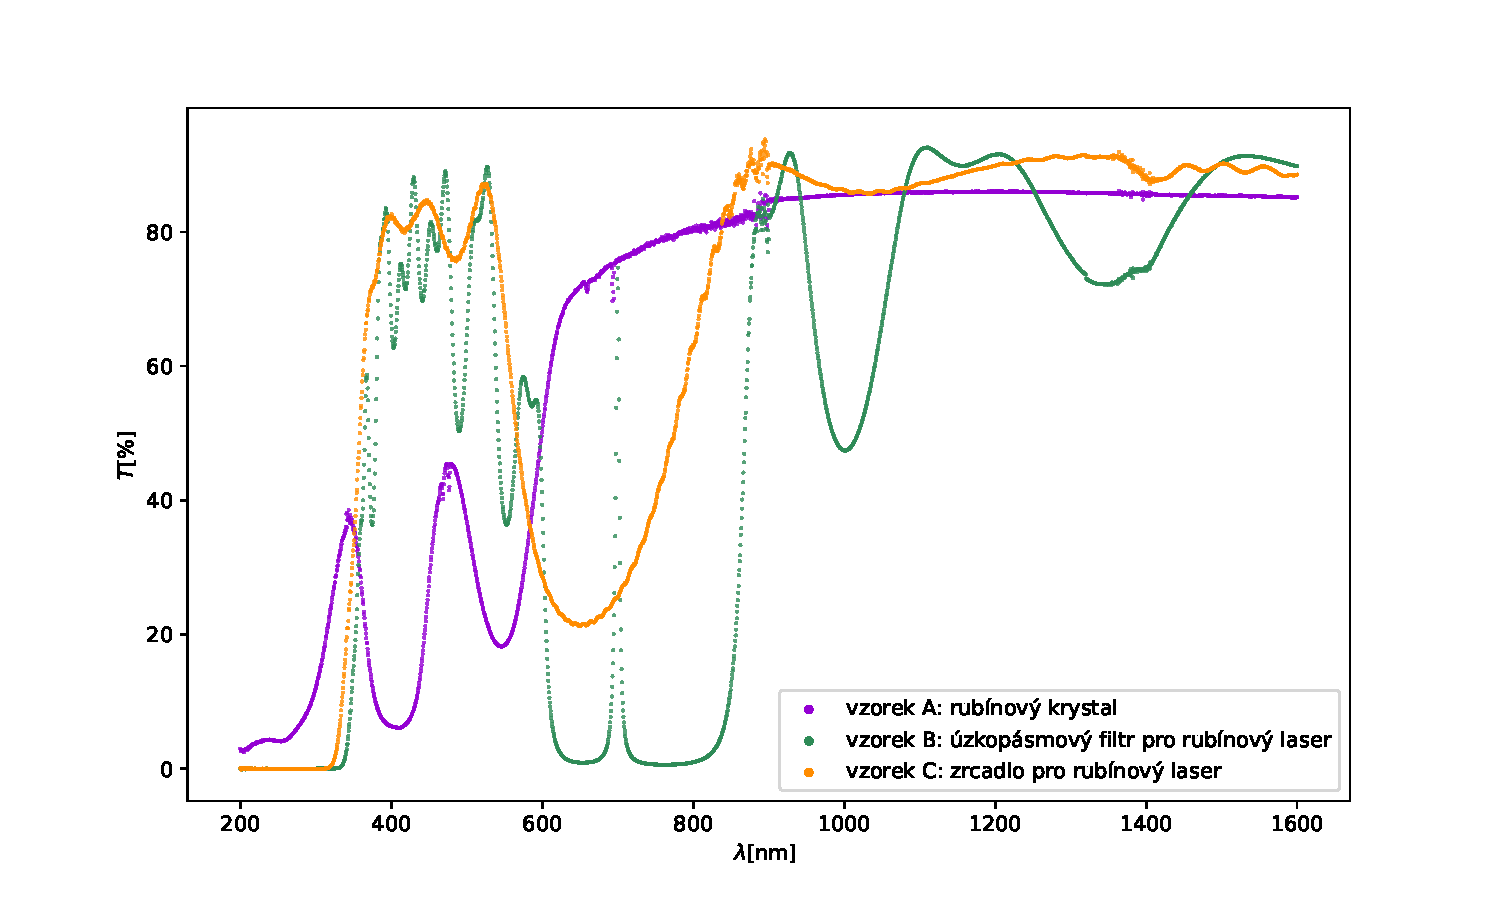
\includegraphics[width=1\textwidth]{img/samples_abc} 
    \caption{Transmisní spektra vzorků A, B a C.}
    \label{fig:abc} %interní popis obrázku
\end{figure}  

\begin{figure}[!hbt]
  \centering
    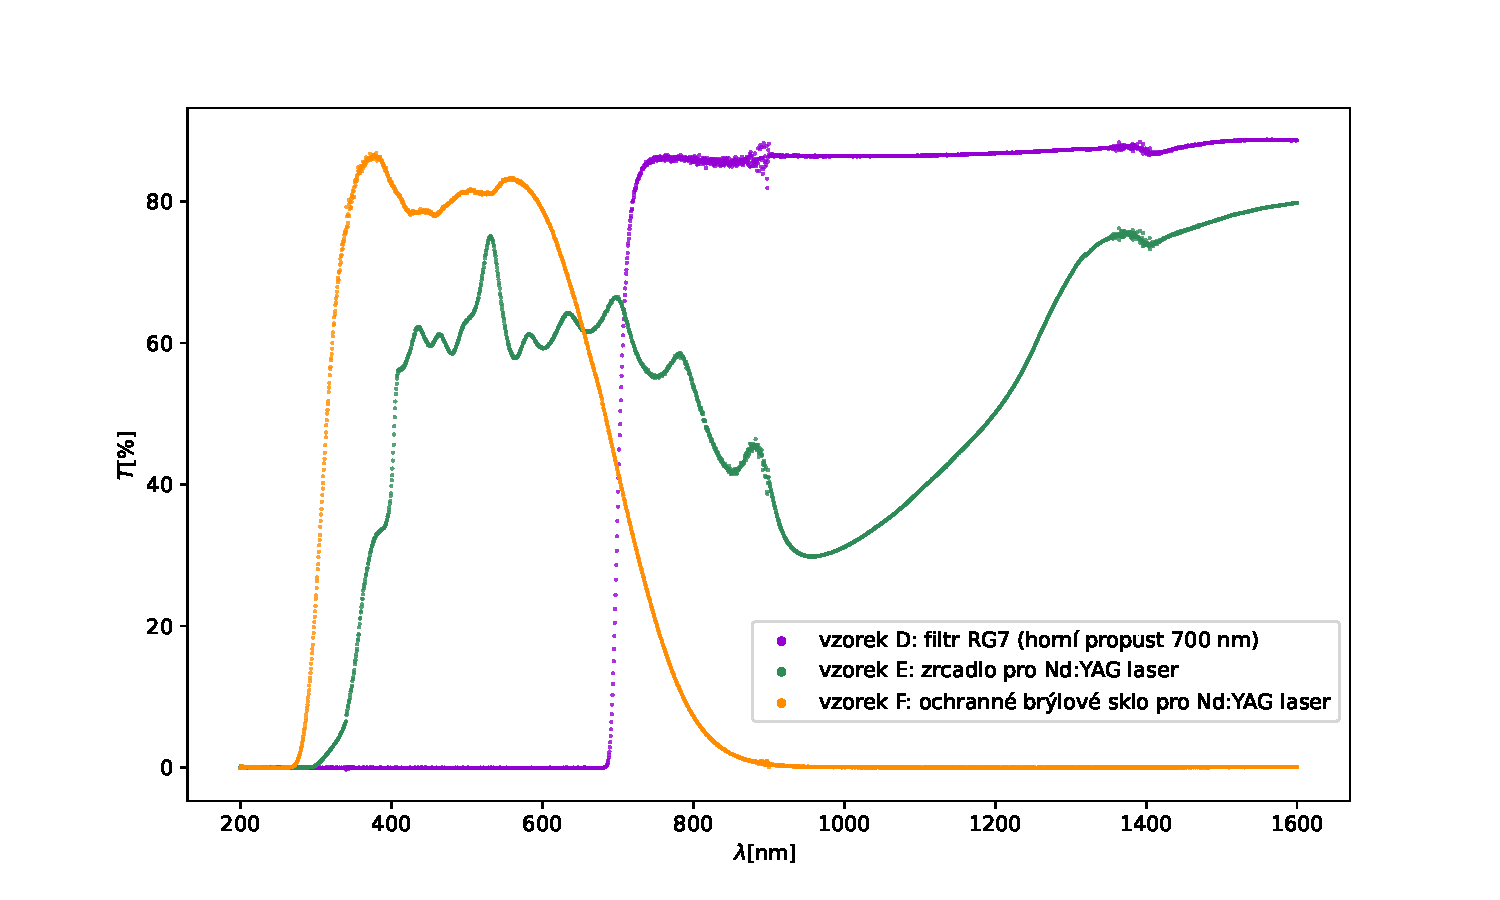
\includegraphics[width=1\textwidth]{img/samples_def} 
    \caption{Transmisní spektra vzorků D, E a F.}
    \label{fig:def} %interní popis obrázku
\end{figure}  

\begin{figure}[!hbt]
  \centering
    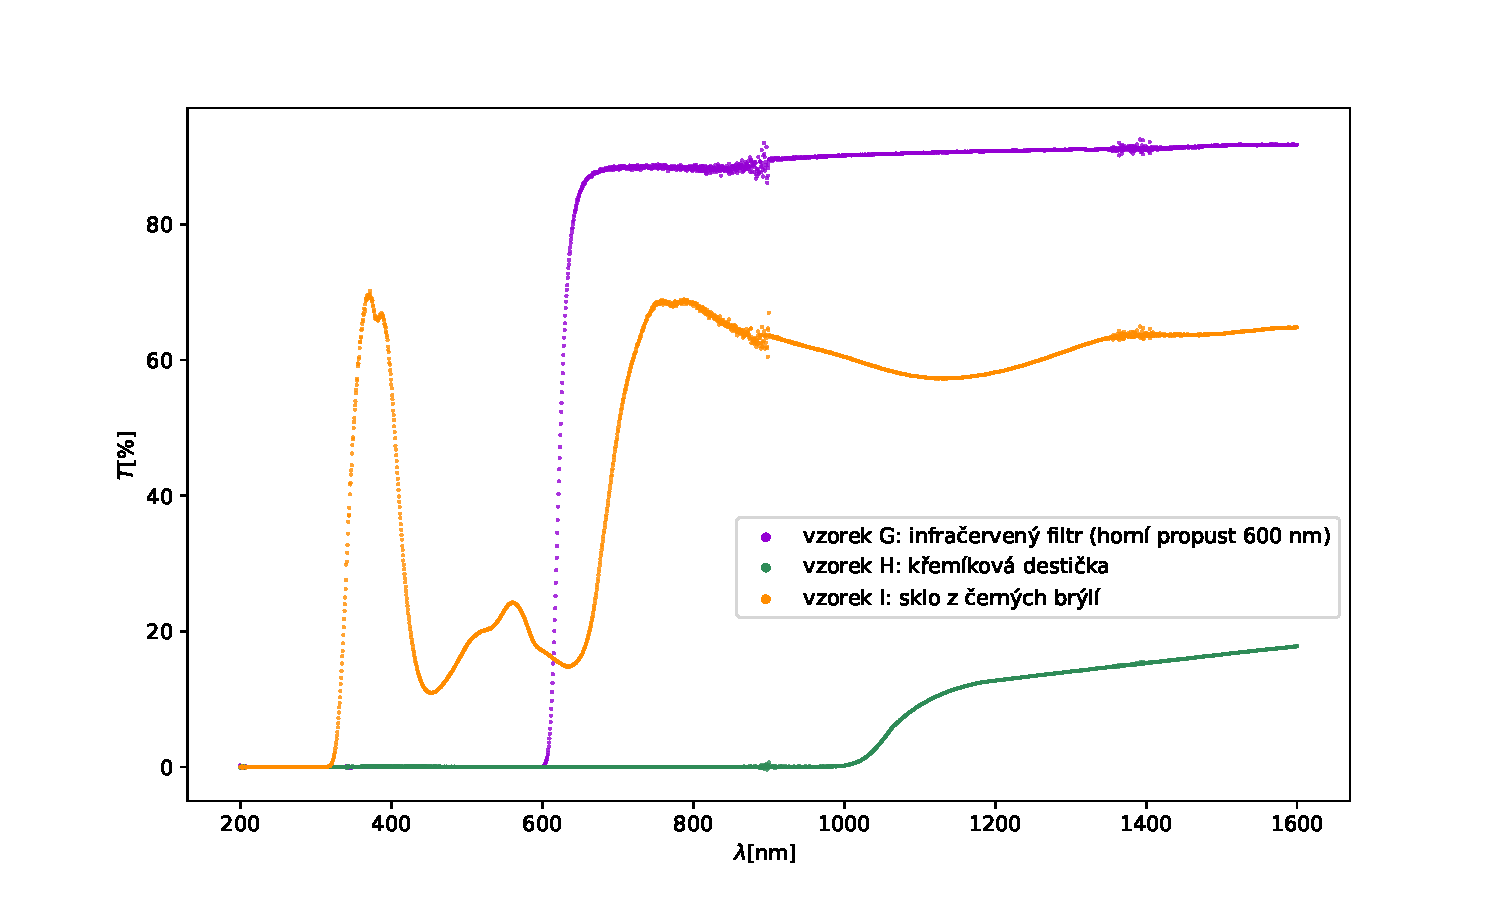
\includegraphics[width=1\textwidth]{img/samples_ghi} 
    \caption{Transmisní spektra vzorků G, H a I.}
    \label{fig:ghi} %interní popis obrázku
\end{figure}  

\begin{figure}[!hbt]
  \centering
    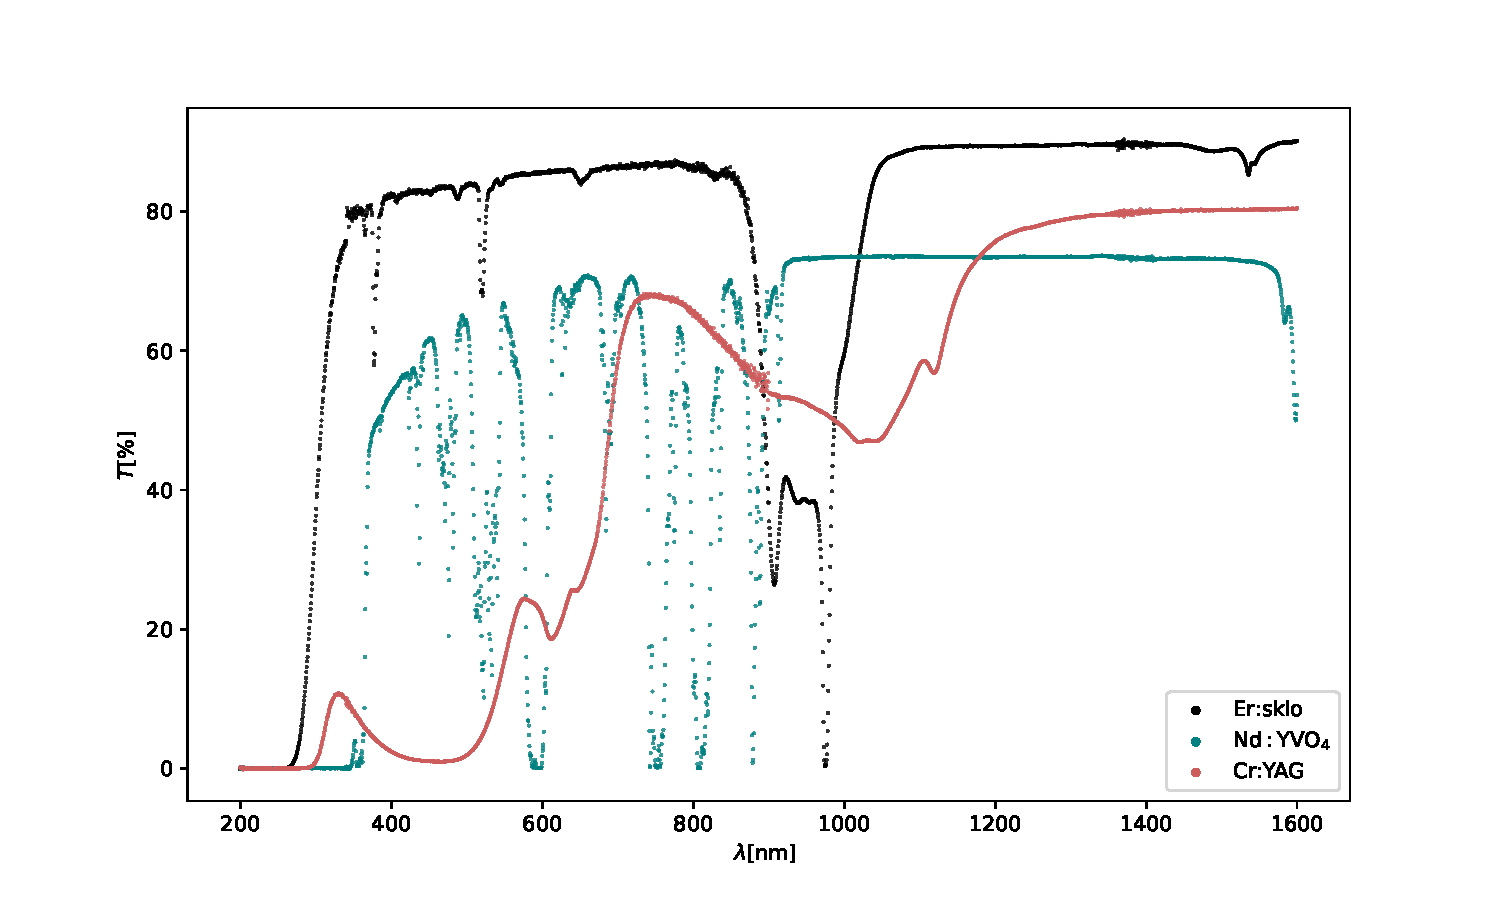
\includegraphics[width=1\textwidth]{img/samples_krystaly.pdf} 
    \caption{Transmisní spektra vzorků laserových krystalů.}
    \label{fig:las} %interní popis obrázku
\end{figure} 
	
	
	\subsection{Dielektrický úzkopásmový filtr pro rubínový laser}
	Šířku transmisního pásu jsme určili jako $\Delta\lambda=11,3\, \mathrm{nm}$ a vlnovou délku pro maximální transmitanci jako $\lambda_{\mathrm{max}}=700\,\mathrm{nm}$. Priblížení transmisního peaku je na obr.~\ref{fig:rubin_filtr}

\begin{figure}[!hbt]
  \centering
    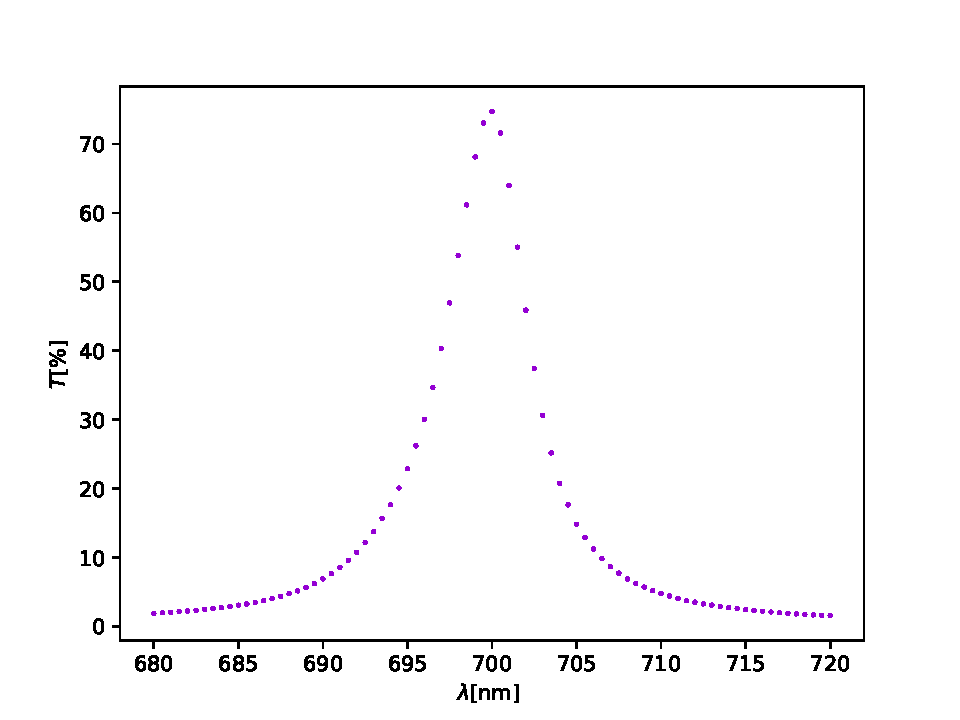
\includegraphics[width=1\textwidth]{img/peak_filtr_rubin.pdf} 
    \caption{Transmisní peak dielektrického úzkopásmového filtr pro rubínový laser v oblasti kolem 694 nm.}
    \label{fig:rubin_filtr} %interní popis obrázku
\end{figure} 
	
	\subsection{Filtr RG7}
	Vlnovou délku, pro kterou je transmise rovna $T=0,5$ jsme určili jako $\lambda_{1/2}=703,5\,\mathrm{nm}$.
	
	\subsection{Rubínový krystal}
	Jednotlivá maxima absorpce $\lambda_{\mathrm{max}}$ a jim příslušné šířky absorpčních pásů $\Delta\lambda$ a koeficienty interní absorpce $\alpha$ se nachází v Tab. \ref{tab:absorpce}.
\begin{table}[!hbt]
\centering
	\begin{tabular}{|c|c|c|}
		\hline
		$\lambda_{\mathrm{max}}$[nm] & $\Delta\lambda$[nm] & $\alpha[\mathrm{cm^{-1}}]$ \\ \hline\hline
		410,0 & 162,4 & 2,47\\ \hline
		545,5 & 142,3 &1,50\\ \hline
		693,0 & 5,5 & 0,32\\ \hline
	\end{tabular}
	\caption{Polohy a šířky jednotlivých maxim absorpce.}
	\label{tab:absorpce}
\end{table}
Absorpční pík na 693 nm odpovídá vlnové délce zářivého přechodu při generování laserového záření. Z toho, že k absorpci na této vlnové délce dochází, soudíme, že se jedná o tříhladinový energetický systém.
\begin{figure}[!hbt]
  \centering
    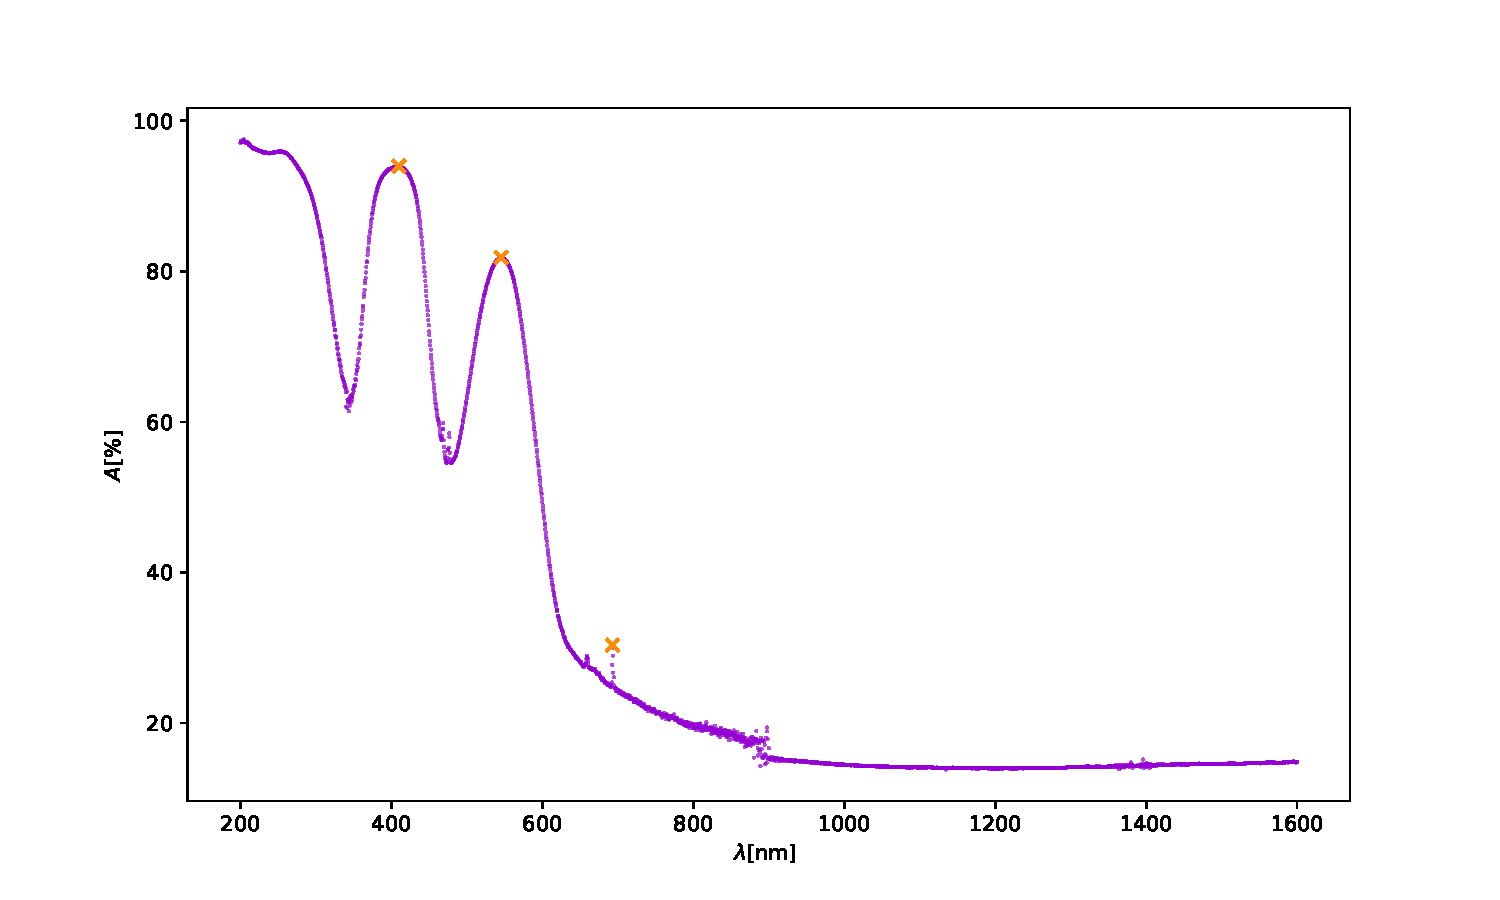
\includegraphics[width=1\textwidth]{img/absorpce_rubin.pdf} 
    \caption{Absorpční spektrum rubínového krystalu s vyznačenými peaky. Ztráty způsobené odrazem byly zanedbány.}
    \label{fig:absorpce_rubin} %interní popis obrázku
\end{figure} 
	

	
	\subsection{Zrcadlo pro Nd:YAG laser}	
	Vzhledem k tomu, že transmise kolem 1 mikrometru je stále ještě kolem 30 \%, pak je vyloučeno, aby reflektivita byla >98 \%. Transmise na 808 nm je zhruba 50 \%, tedy zrcadlo není vhodné pro čerpání diodou.
	
	\subsection{Zrcadlo pro rubínový laser}
	Transmise pro vlnové délky kolem 695 nm je příliš vysoká -- kolem 30 \%, tedy zrcadlo není použitelné jako HR zrcadlo pro tuto vlnovou délku.
	
	\subsection{Laserový krystal Nd:YVO4}
	Transmisní spektrum odhalilo peaky absorpce na vlnových délkách 808 nm, 835 nm, 878 nm a 888 nm. K čerpání pomocí laserových diod je nejčastěji používáno maximum na 808 nm, ovšem někdy se používá i čerpání vlnovou délkou 878 nm. Šířky těchto peaků (a tedy i optimální šířka pásma použité diody) odpovídá 24 nm pro čerpání na 808 nm a 16 nm pro čerpání na 878 nm.\\
	
	Vlnové délky laserového záření generované krystalem $\mathrm{Nd:YVO_4}$ jsou 914 nm, 1064 nm a 1342 nm. Na 914 nm je znatelný pokles transmise, na ostatních zmíněných vlnových délkách ne. Pro vlnovou délku 914 nm se tedy jedná o tříhladinivý systém, pro 1064 a 1342 nm jde o systém čtyřhladinový (ani jedna z hladin, mezi kterými dochází k zářivému přechodu ve čtyřhladinovém laseru, není stabilní a absorpce je proto neppravděpodobná).
	\begin{figure}[!hbt]
  \centering
    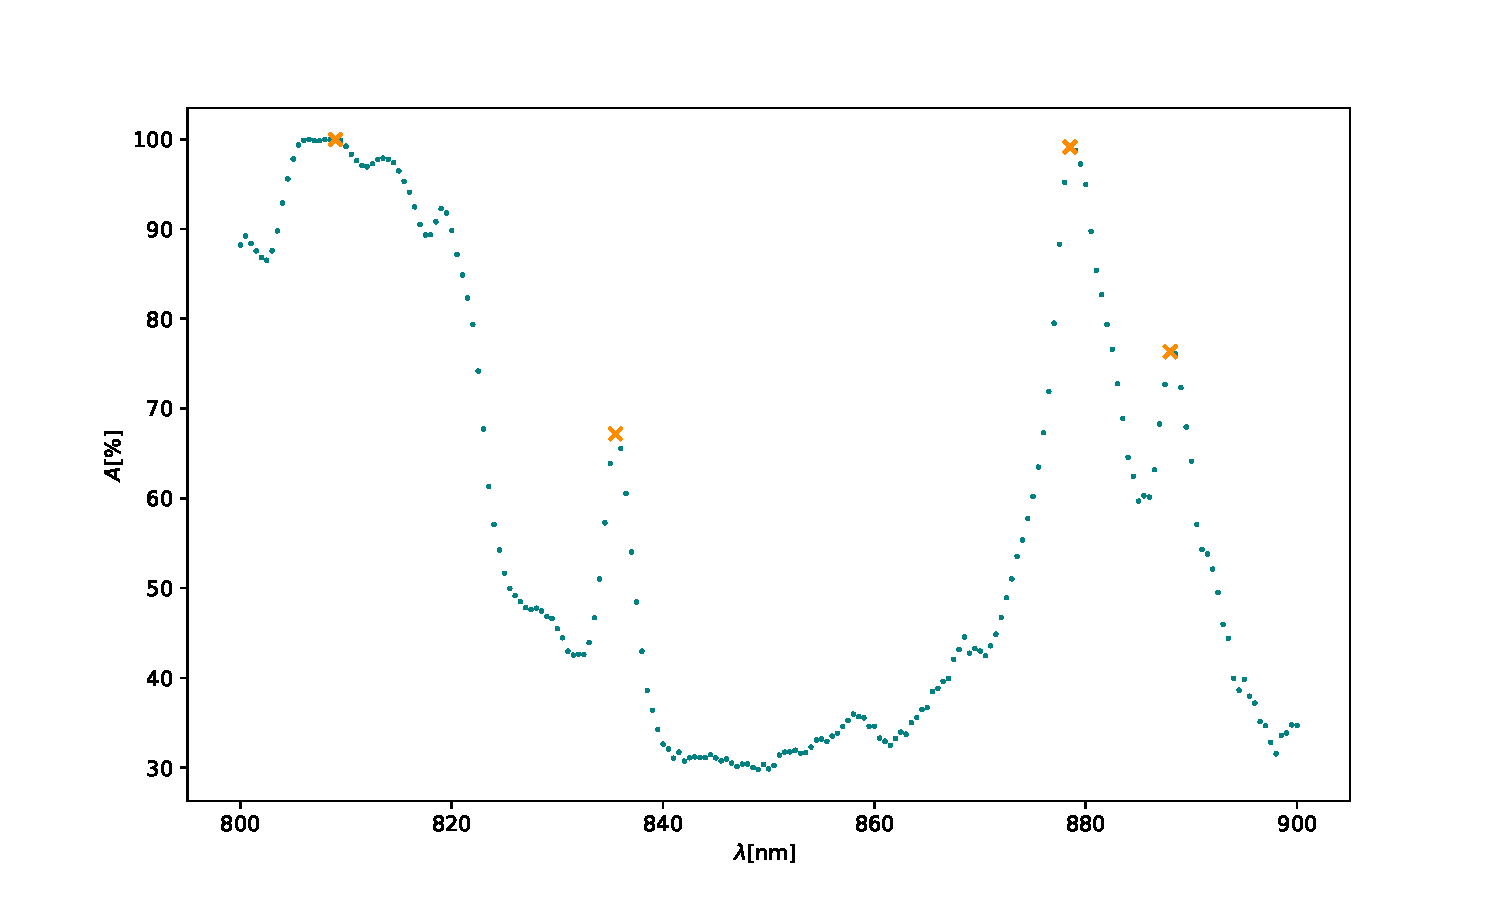
\includegraphics[width=1\textwidth]{img/absorpce_NdYVO.pdf} 
    \caption{Peaky absorpce krystalu $\mathrm{Nd:YVO_4}$ v rozmezí 800 - 900 nm. Ztráty způsobené odrazem byly zanedbány.}
    \label{fig:absorpce_NdYVO} %interní popis obrázku
\end{figure} 

\begin{figure}[!hbt]
  \centering
    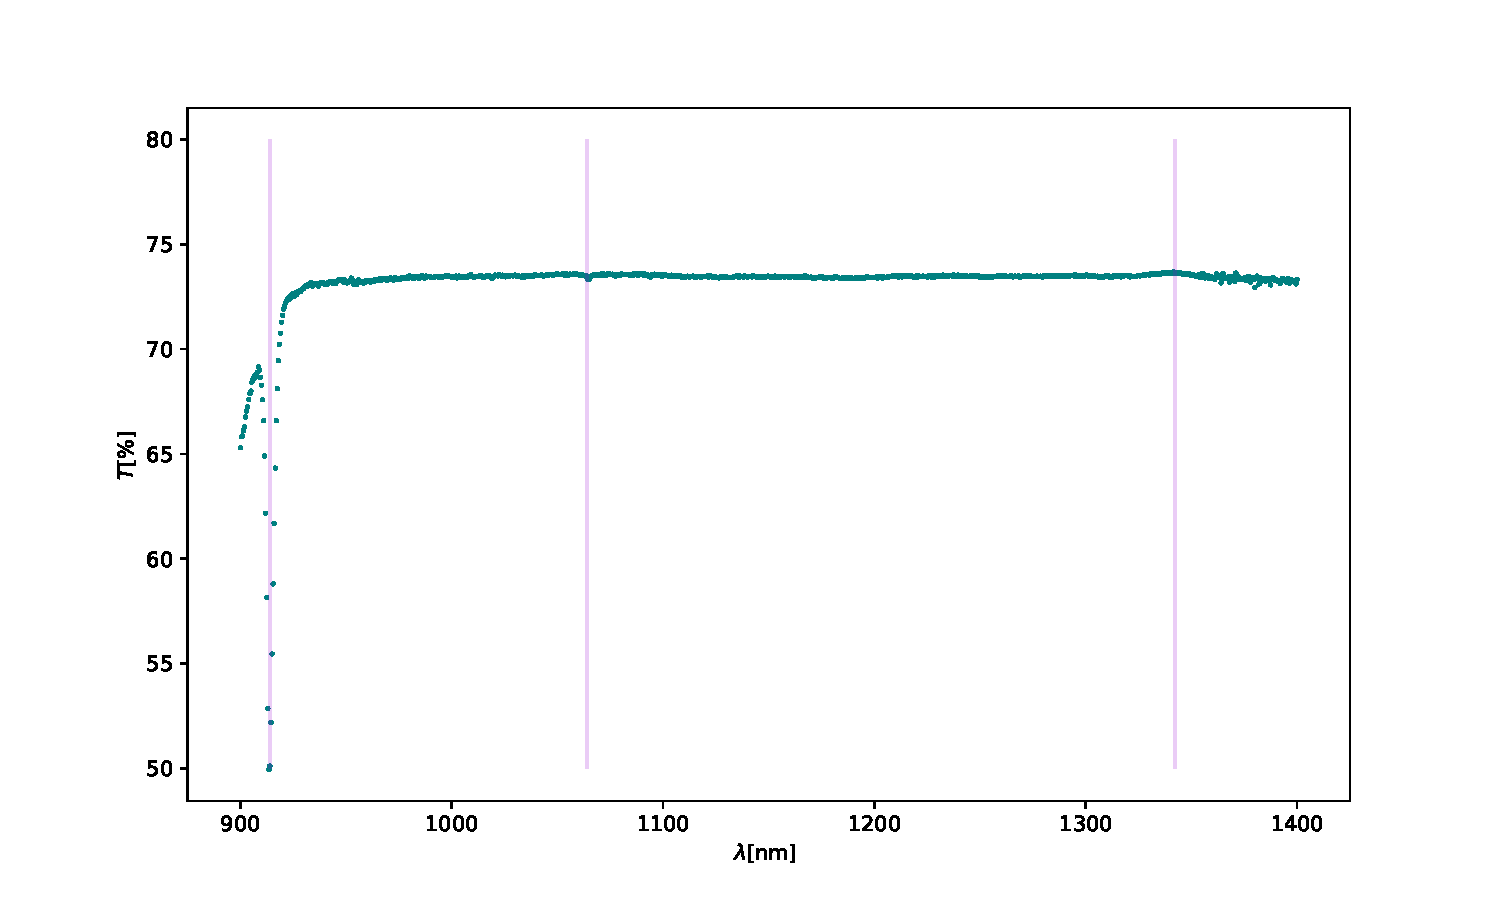
\includegraphics[width=1\textwidth]{img/las_NdYVO.pdf} 
    \caption{Transmisní spektrum krystalu $\mathrm{Nd:YVO_4}$ s vyznačenými vlnovými délkami zářivých přechodů při generaci laserového záření.}
    \label{fig:absorpce_NdYVO} %interní popis obrázku
\end{figure} 
	
	
	\subsection{Laserový krystal Er:sklo}
	Z transmisního spektra jsou patrné dvě absorpční maxima, první okolo 908 nm a druhé okolo 975 nm. K čerpání se nejčastěji používají vlnové délky kolem 975 nm. Šířka tohoto absorpčního peaku je 25 nm, což je tedy také optimální spektrální šířka použité čerpací diody. 
	Er:sklo lasery produkují laserové záření na vlnových délkách 1535, 1544 a 1562 nm. V transmisním spektru je pozotovatelný pokles transmisivity na 1535 nm  1544 nm. Na těchto vlnových délkách se tedy jedná o tříhladinový systém, zbylá vlnová délka 1562 nm odpovídá čtyřhladinovému systému.
	
\begin{figure}[!hbt]
  \centering
    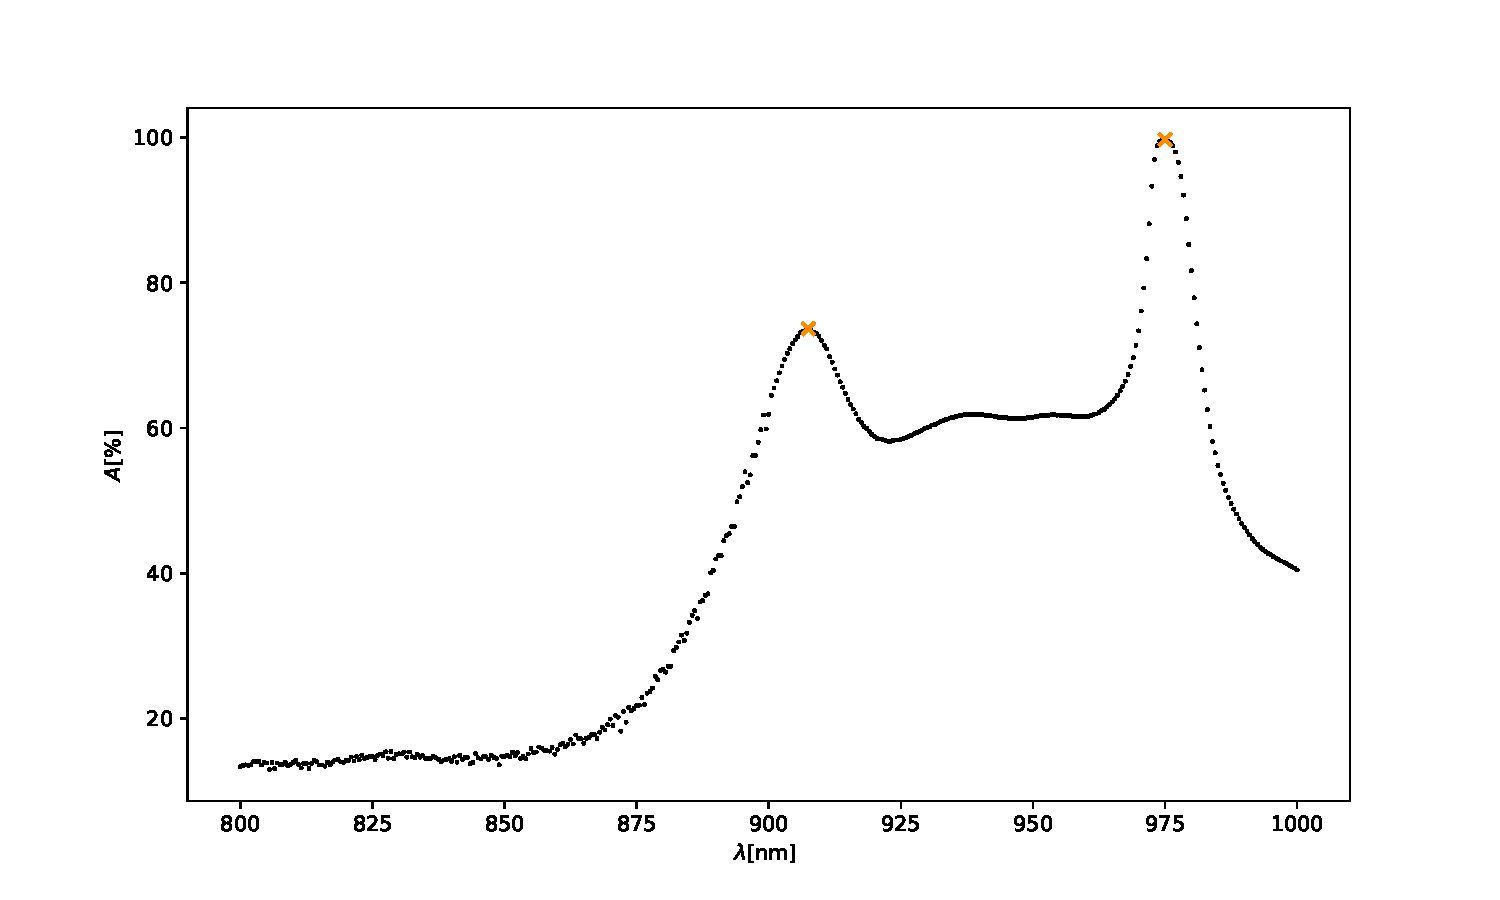
\includegraphics[width=1\textwidth]{img/absorpce_Er_sklo.pdf} 
    \caption{Absorpční peaky krystalu ER:sklo v rozmezí 800 - 1000 nm. Ztráty způsobené odrazem byly zanedbány.}
    \label{fig:absorpce_Ersklo} %interní popis obrázku
\end{figure} 

\begin{figure}[!hbt]
  \centering
    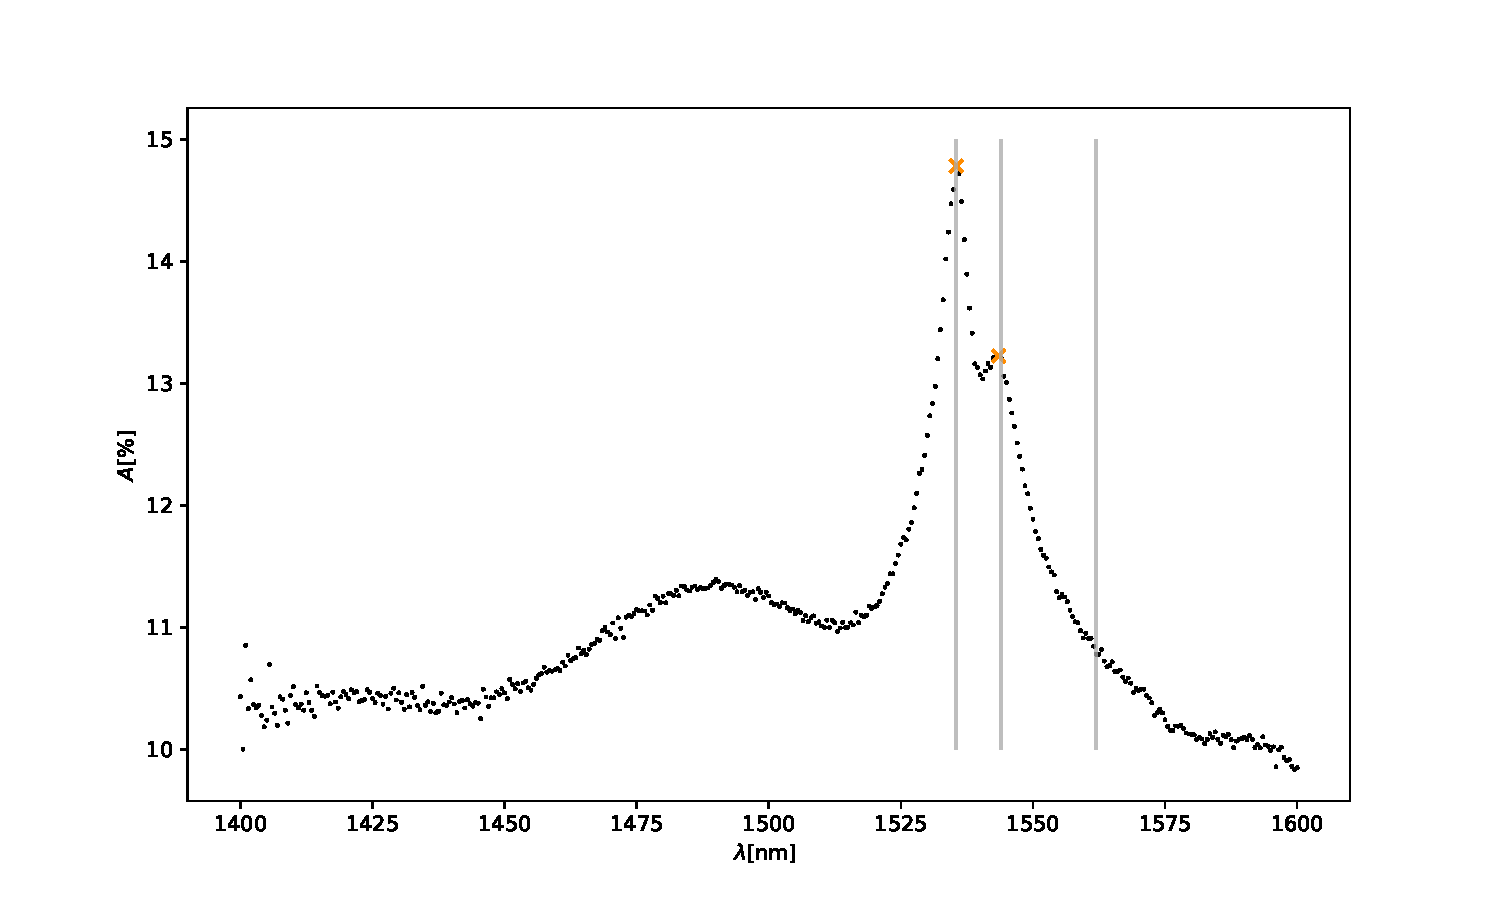
\includegraphics[width=1\textwidth]{img/las_Er_sklo.pdf} 
    \caption{Absorpční spektrum krystalu ER:sklo v blízkosti vlnových délek zářivých přechodů při generaci laserového záření. Ztráty způsobené odrazem byly zanedbány.}
    \label{fig:las_Ersklo} %interní popis obrázku
\end{figure} 
\newpage
	\subsection{Krystal Cr:YAG}
	V laserové technice se Cr:YAG používá jako saturovatelný absorbér pro Nd:YAG lasery, dále může sloužit jako aktivní médium pro laditelný laser na vlnových délkách mezi 1350 a 1550 nm a také je možné jej použít pro generování femtosekundových pulsů.
	Tloušťka měřeného krystalu byla 1,04 mm a interní absorpční koeficient $\alpha_{1060}$ pro vlnovou délku 1060 nm je roven přibližně 6,8 $\unit{cm^{-1}}$
 			

	\subsection{Vliv neúplného zakrytí plochy měřicího svazku vzorkem}
		Při měření vzorků menších, než je plocha měřícího svazku, kolem vzorku na detektor projde světlo, které by jinak vzorkem bylo absorbováno či odraženo. Kvůli tomu dojde ke zkreslení hodnot transmisivity, zejména pro vlnové délky, na kterých má vzorek transmisivitu nízkou. 
% ----------------------------------------------------------------------
%  Diskuse - obsahuje komentář k jednotlivým výsledkům, porovnání s očekáváním/tabulkovými hodnotami, zdroje především systematických chyb měření, návrh na zlepšení výsledků,...
% ----------------------------------------------------------------------			
%\section{Diskuse}			

% ----------------------------------------------------------------------
%  Závěr - stručně a jasně shrnout splněné cíle měření, úkoly a výsledky měření
% ----------------------------------------------------------------------
			
%\section{Závěr}



